
\subsection{China Electronic Toll Colleciton}
China memiliki masyarakat yang sangat banyak dan setiap masyarakat memiliki sekurang kurangnya satu kendaraan. Seiring bertambah nya masyarakat di China, maka jalanan yang ada di China akan semakin penuh dengan kendaraan yang akan menghasilkan kemacetan terutama pada tol bagian pembayaran. Untuk mengatasi masalah ini China menggunakan \textit{Electronic Toll Colleciton (ETC)} yang di integrasikan dengan setiap kendaraan untuk mempercepat proses ini \parencite{penelitianterkait1}.

China menggunakan KubeEdge untuk melakukan proses \textit{deployment} \textit{ETC} untuk 100,000 \textit{nodes} dengan total 500,000 aplikasi yang diluncurkan menggunakan KubeEdge tersebar untuk 29 dari 34 provinsi. Proses \textit{deployment} dilakukan secara otomatis dengan membuat sistem \textit{workflow engine} pada kubernetes sehingga proses \textit{deployment} dapat dilakukan dengan cepat dan mudah. Dengan menggunakan metode ini sistem pembayaran tol di China menjadi 10x lebih cepat dari sebelumnya \parencite{penelitianterkait1}.

\begin{figure}[ht]
  \centering
  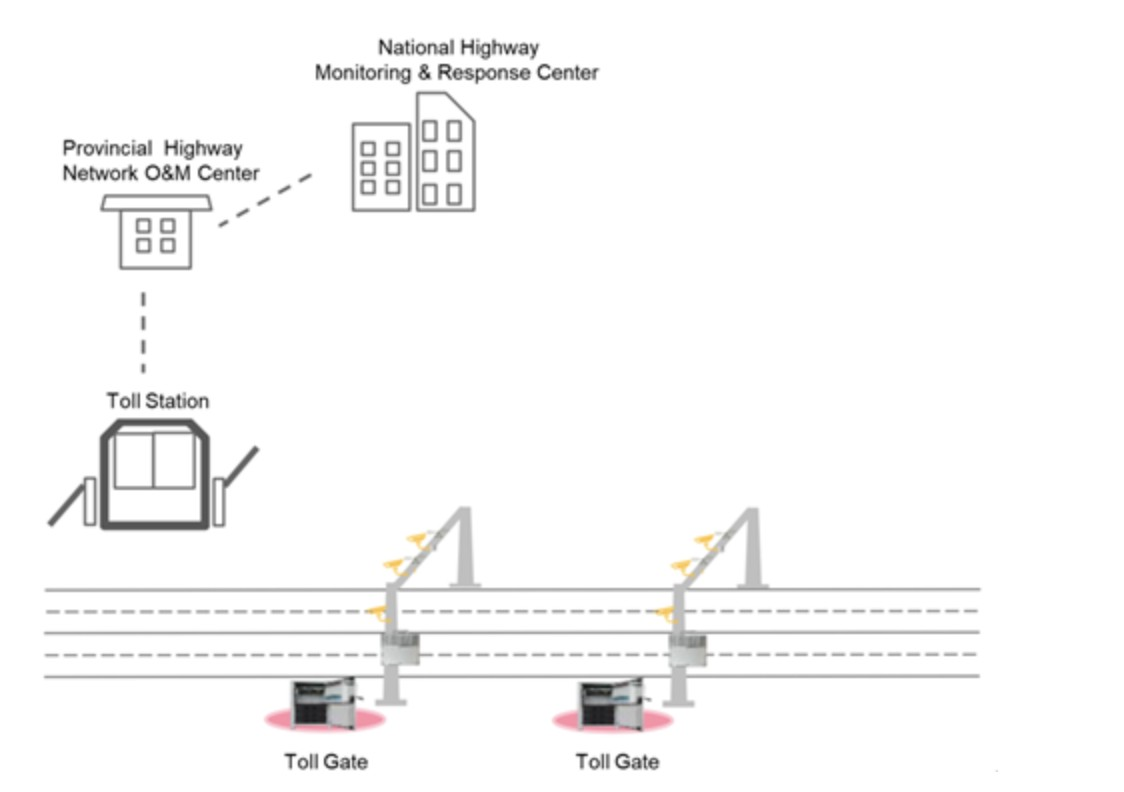
\includegraphics[width=0.8\textwidth]{resources/chapter-2/china-highways.jpg}
  \caption{Implementasi Sistem \textit{ETC} di China \parencite{penelitianterkait1}}
  \label{fig:china-highways}
\end{figure}

\begin{figure}[ht]
  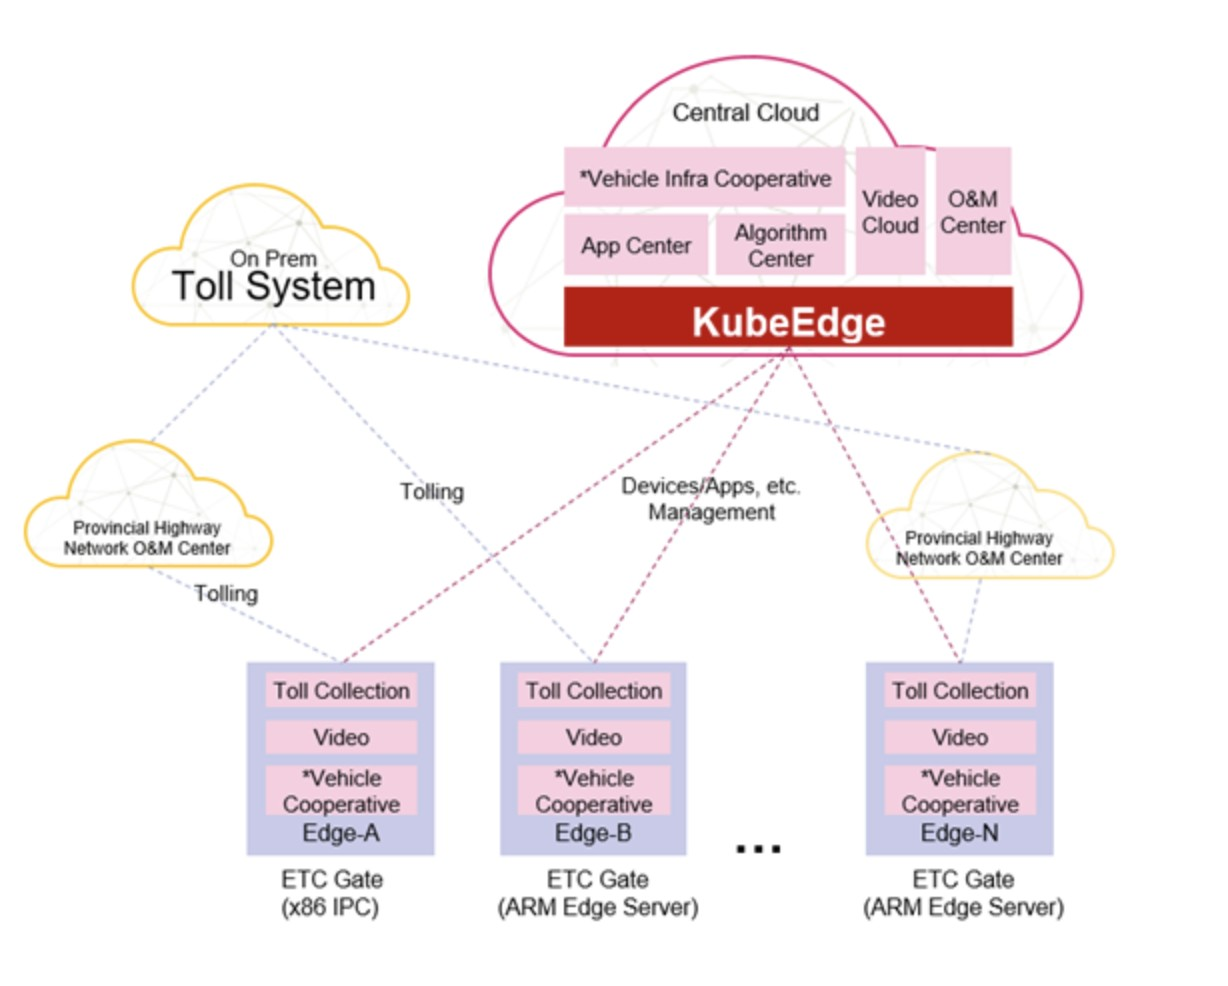
\includegraphics[width=0.8\textwidth]{resources/chapter-2/arsitektur-china-highways.jpg}
  \caption{Arsitektur Sistem \textit{ETC} di China \parencite{penelitianterkait1}}
  \label{fig:architecture-china-highways}
\end{figure}